% 原 Word 的流程图作为图片保留其线型、填色和文字位置。
\clearpage
\begingroup\ecjtuwordgridfalse
\vspace*{-19.7545bp}
\begin{figure}[H]
\centering
\captionsetup{skip=4.1935bp}
\hspace*{-0.088bp}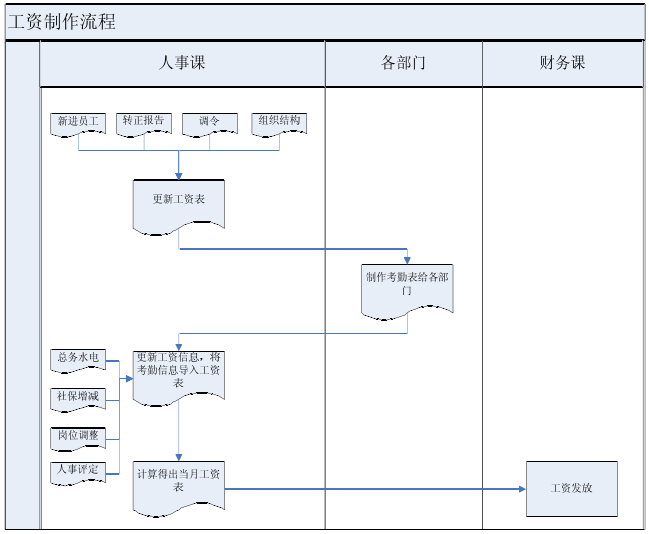
\includegraphics[width=369bp,height=303.6bp]{assets/salary-flow.png}
\caption{工资制作流程图}\label{fig:salary}
\end{figure}
\vspace{-17.43bp}
\normaltemplatehints
\templatehint{\xeCJKsetup{PunctStyle=quanjiao}\mbox{\xeCJKsetup{PunctStyle=plain}（}论文中\guidanceem{图}\hspace{6bp}的画法，注意以下几点：1\hspace{6bp}图要用word画，或者采用粘贴方式，不能使用截\linebreak
图方式，否则打印出来图的效果很不清晰。2\hspace{6bp}\guidanceem{图的标题}\hspace{6bp}要写在\guidanceem{图的下方}，\guidanceem{居中}，用\hspace{5.52bp}\guidanceem{5\hspace{5.52bp}号}\linebreak
\guidanceem{黑体字}。3\hspace{6bp}\guidanceem{图中的文字}采用\guidanceem{5号宋体字}。4\hspace{6bp}\guidanceem{每章}的所有图采用\guidanceem{顺序编号}，如图3-1，图3-2\linebreak
等）}

\vspace{11.71bp}
\begin{table}[H]
\captionsetup{skip=0.03bp}
\caption{工资管理问题点}\label{tab:salary}
\tablefont
\renewcommand{\arraystretch}{1}
\setlength{\tabcolsep}{5.16bp}
\setlength{\arrayrulewidth}{0.48bp}
\setbox\strutbox=\hbox{\ecjtuwordstrut{13.56}{6}}
\hspace*{21.36bp}\begin{tabular}{|p{48.596bp}|p{61.23bp}|p{132.74bp}|p{97.71bp}|}
\hline
涉及点 & 目前做法 & 存在问题 & 希望改善\\\hline
考勤 & 各部门汇总 & 考勤存在虚报、错误时无法核对，导致错误。 & 考勤准确\\\hline
工资计算 & 凭公式计算 & 灵活，\hspace{-4.68bp}但易出错，\hspace{-4.68bp}且不易检查。 & {\xeCJKsetup{CJKglue=\hskip0.36bp}固定某些必要内容，}\newline 使出错率降低。\\\hline
人员信息 & {\xeCJKsetup{CJKglue=\hskip2.1bp}以批注的形}\newline 式予以提醒 & 易出现遗漏现象，且人事系统与工资系统无法相对应。 & {\xeCJKsetup{CJKglue=\hskip0.33bp}\XeTeXcharclass"FF0C=1\relax 使用同一系统，达到}\newline 信息共享目的。\\\hline
\end{tabular}
\end{table}
\vspace{1.95bp}
\templatehint{\xeCJKsetup{PunctStyle=quanjiao}\mbox{\xeCJKsetup{PunctStyle=plain}（}论文中\guidanceem{表}\hspace{6bp}的画法，注意以下几点：1\hspace{6bp}表要用word画，不能使用截图方式，否则打印出\linebreak
来效果很不清晰。2\hspace{6bp}\guidanceem{表的标题}\hspace{6bp}要写在\guidanceem{表的上方}，\guidanceem{居中}，用\guidanceem{5号黑体字}。3\hspace{6bp}\guidanceem{表中的文字}\hspace{6bp}采\linebreak
用\guidanceem{5号宋体字}。4\hspace{6bp}\guidanceem{每章}\hspace{6bp}的所有表采用\hspace{6bp}\guidanceem{顺序编号}，如表3-1，表3-2等）}
\endgroup
